% Figure snippets for main.tex

\begin{figure}[t]
\centering
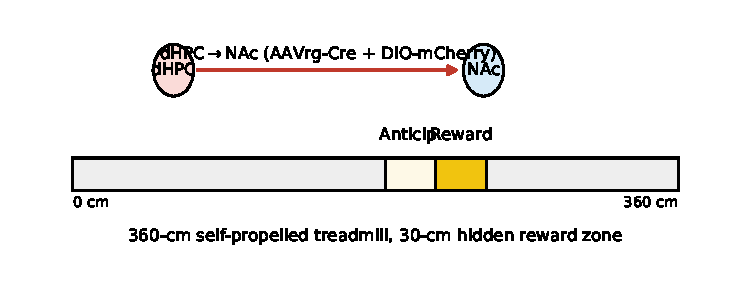
\includegraphics[width=0.95\linewidth]{figures/fig5_schematic.pdf}
\caption{\textbf{Projection-specific imaging during a spatial reward task.}
Mice ran on a 360-cm self-propelled treadmill with a 30-cm hidden reward zone
preceded by a 30-cm anticipation zone. NAc-projecting dHPC neurons were
labeled by injecting retrograde AAVrg-pgk-Cre into NAc together with
Cre-dependent AAV5-hSyn-DIO-mCherry into dHPC of Thy1-GCaMP6s mice, enabling
dual-color two-photon imaging of pan-neuronal GCaMP6s and projection-defined
mCherry.}
\label{fig:schematic}
\end{figure}

\begin{figure}[t]
\centering
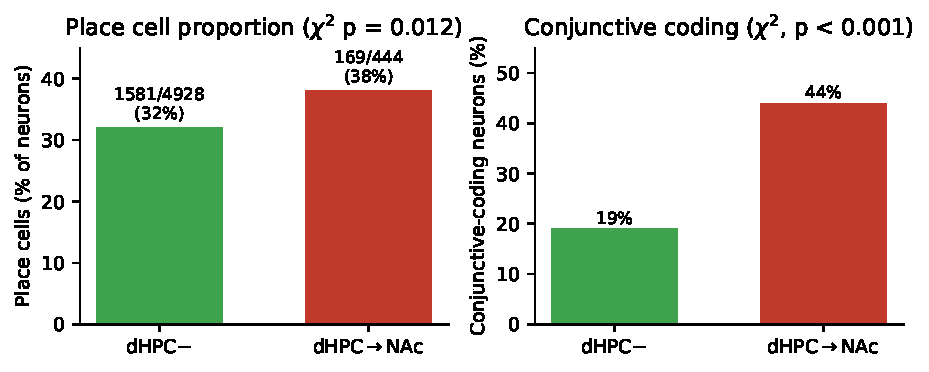
\includegraphics[width=0.95\linewidth]{figures/fig1_place_conjunctive.pdf}
\caption{\textbf{NAc-projecting dHPC neurons are enriched for place cells and
for conjunctive coding.} Left: proportion of place cells is higher in
dHPC$\rightarrow$NAc (169/444, 38\%) than in dHPC$-$ (1{,}581/4{,}928, 32\%;
$\chi^2$, $p = 0.012$). Right: a generalized linear model classifies 44\% of
dHPC$\rightarrow$NAc neurons as conjunctive coders of space, velocity and
licking, versus 19\% of dHPC$-$ neurons ($p<0.001$).}
\label{fig:place_conj}
\end{figure}

\begin{figure}[t]
\centering
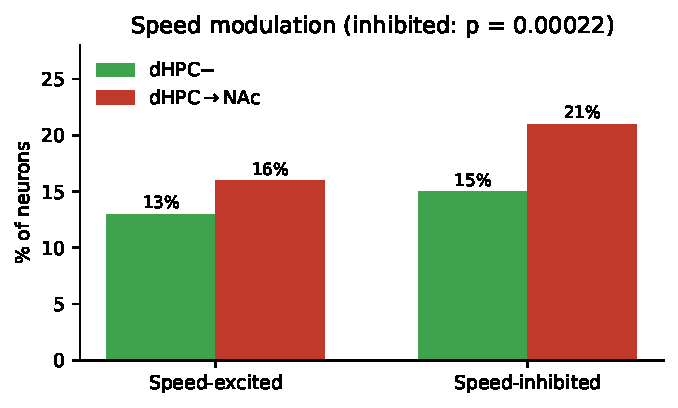
\includegraphics[width=0.85\linewidth]{figures/fig2_speed.pdf}
\caption{\textbf{Speed-inhibited neurons are overrepresented in
dHPC$\rightarrow$NAc.} Proportions of speed-excited neurons are comparable
across populations (13\% vs 16\%, $\chi^2$, $p=0.109$), whereas speed-inhibited
neurons are significantly more frequent in dHPC$\rightarrow$NAc (15\% vs
21\%, $p=0.00022$).}
\label{fig:speed}
\end{figure}

\begin{figure}[t]
\centering
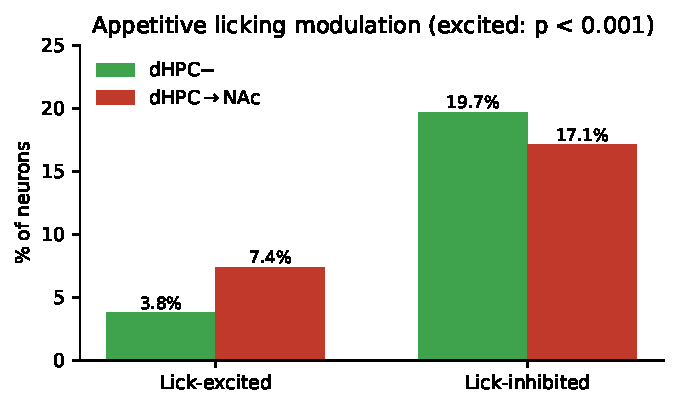
\includegraphics[width=0.85\linewidth]{figures/fig3_lick.pdf}
\caption{\textbf{Appetitive licking-excited neurons are overrepresented in
dHPC$\rightarrow$NAc.} Lick-inhibited proportions are indistinguishable
(19.7\% vs 17.1\%, $p=0.20$), while lick-excited proportions are nearly
doubled in dHPC$\rightarrow$NAc (3.8\% vs 7.4\%, $p<0.001$).}
\label{fig:lick}
\end{figure}

\begin{figure}[t]
\centering
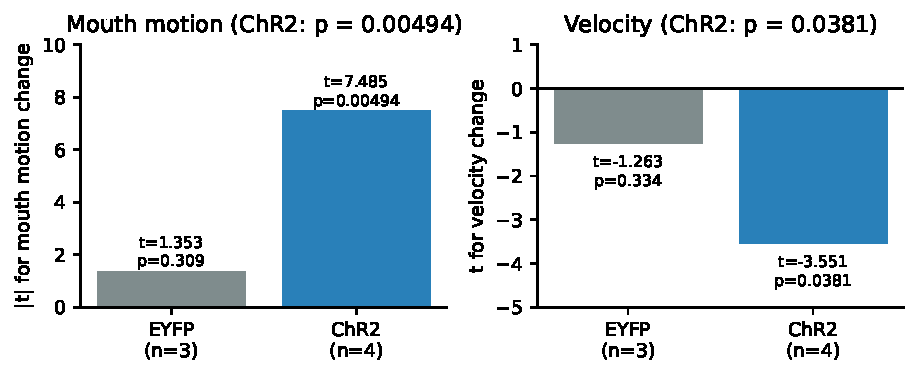
\includegraphics[width=0.95\linewidth]{figures/fig4_opto.pdf}
\caption{\textbf{Optogenetic activation of dHPC terminals in NAc evokes
mouth movement and deceleration.} Paired $t$-tests comparing pre-
vs.\ during-stimulation epochs: mouth motion increases only in ChR2 mice
($t(3)=7.485$, $p=0.00494$) but not in EYFP controls ($t(2)=1.353$,
$p=0.309$); velocity decreases only in ChR2 mice ($t(3)=-3.551$,
$p=0.0381$) but not EYFP ($t(2)=-1.263$, $p=0.334$).}
\label{fig:opto}
\end{figure}
